\documentclass[fleqn,10pt]{wlscirep}
\usepackage[utf8]{inputenc}
\usepackage[T1]{fontenc}
\usepackage{siunitx}
\usepackage{subcaption}
\usepackage{xargs}  % Use more than one optional parameter in a new commands
\usepackage[colorinlistoftodos,prependcaption]{todonotes}

\sisetup{locale=US,group-minimum-digits=5,group-separator={,}}

\newcommandx{\alltodo}[2][1=]{\todo[author=Everyone,linecolor=red,backgroundcolor=red!25,bordercolor=red,#1]{#2}}
\newcommandx{\mctodo}[2][1=]{\todo[author=Matt,linecolor=blue,backgroundcolor=blue!25,bordercolor=blue,#1]{#2}}
\newcommandx{\comment}[2][1=]{\todo[author=Comment,linecolor=lime,backgroundcolor=lime!25,bordercolor=lime,#1]{#2}}
\newcommandx{\arhtodo}[2][1=]{\todo[author=Adam,linecolor=purple,backgroundcolor=purple!25,bordercolor=purple,#1]{#2}}

\title{A preprocessed open diffusion derivatives dataset from the Healthy Brain Network}

\author[1,*$\dagger$]{Adam Richie-Halford}
\author[2,$\dagger$]{Matthew Cieslak}
\author[4]{Lei Ai}
\author[5]{Sendy Caffarra}
\author[4]{Alexandre R. Franco}
\author[5]{Iliana Karipidis}
\author[3]{John Kruper}
\author[5]{Barbara Avelar Pereira}
\author[5]{Ethan Roy}
\author[2]{Valerie J. Sydnor}
\author[5]{Jason Yeatman}
\author[4]{Michael Milham}
\author[6]{Jul\_dugre}
\author[6]{amandamcgow}
\author[6]{SimonMB}
\author[6]{Nabbott}
\author[6]{AmjadSamara}
\author[6]{Shannon Grogans}
\author[6]{Zzzdeng}
\author[6]{HamidTurker}
\author[6]{Dragon}
\author[6]{Lshaffe6}
\author[6]{Hilarym}
\author[6]{faskybrain}
\author[6]{RaeYuan}
\author[6]{wanderinggrace}
\author[6]{sofie}
\author[6]{llotter}
\author[6]{valeriejill}
\author[6]{AkiNikolaidis}
\author[6]{Deagaric}
\author[6]{akoz}
\author[6]{summerf}
\author[6]{lindenmp}
\author[6]{mjl0062}
\author[6]{Nevena}
\author[6]{kat\_sh}
\author[6]{LeonF}
\author[6]{anjaue}
\author[6]{utooley1}
\author[6]{adrian\_neurosci}
\author[6]{mattwall}
\author[6]{Griffin SH}
\author[6]{jbourque}
\author[6]{averigiudicessi}
\author[6]{ncolenbi}
\author[6]{vtrip}
\author[6]{MeganHimes}
\author[6]{ti}
\author[6]{floundersmw}
\author[6]{itsyuchao}
\author[6]{jjfc}
\author[6]{Agwiesman}
\author[6]{bhaggerty}
\author[6]{benjamindeleener}
\author[6]{AnthonyJa}
\author[6]{seedyh}
\author[6]{nm\_fibr}
\author[6]{matthew2}
\author[6]{Li}
\author[6]{Gabriel Gonzalez-Escamilla}
\author[6]{Gianpaolo}
\author[6]{Mareike}
\author[6]{arielleered}
\author[6]{gdelap}
\author[6]{elliem}
\author[6]{skorenic}
\author[6]{Mark Wiesman}
\author[6]{SHKohl}
\author[6]{claudiap}
\author[6]{mackenzie}
\author[6]{jaewsong}
\author[6]{guillaume}
\author[6]{sadieneuro}
\author[6]{GuiomarNiso}
\author[6]{PSB}
\author[6]{elorenc}
\author[6]{smarek}
\author[6]{fsayed}
\author[6]{gthf61448}
\author[6]{WendyWang}
\author[6]{dcg2153}
\author[6]{mpeter55}
\author[6]{earoy}
\author[6]{cmich}
\author[6]{ikahhale}
\author[6]{czaj}
\author[6]{JodyFinch11}
\author[6]{albie}
\author[6]{holoships}
\author[6]{ckw84}
\author[6]{Gaga}
\author[6]{ecoffey}
\author[6]{jmayor}
\author[6]{jbryn}
\author[6]{jlurp20}
\author[6]{ShaoshiZ}
\author[6]{slhkam}
\author[6]{ckorponay}
\author[6]{BrunoHeblingVieira}
\author[6]{Yacine Mahdid}
\author[6]{harriet89}
\author[6]{Christian}
\author[6]{JonathanTSchneider}
\author[6]{bennewman}
\author[6]{sidchop}
\author[6]{Smeisler}
\author[6]{roryboyle}
\author[6]{cMadan}
\author[6]{MaryLena}
\author[6]{mkp}
\author[6]{Twelton}
\author[6]{dalez}
\author[6]{hyruuk}
\author[6]{ehhall}
\author[6]{jlhanson5}
\author[6]{smomara}
\author[6]{EvrenOzarslan}
\author[6]{ctw}
\author[6]{mollyr}
\author[6]{NChaku}
\author[6]{iliazaharov}
\author[6]{askeller}
\author[6]{clh64}
\author[6]{flat\_brainer}
\author[6]{H Farmer}
\author[6]{Jacobjcrouse}
\author[6]{Ryguy}
\author[6]{VincentBottom}
\author[6]{aomary}
\author[6]{aojha7}
\author[6]{wanderine}
\author[6]{Kahini}
\author[6]{bc1115}
\author[6]{adam}
\author[6]{sasims}
\author[6]{anovan}
\author[6]{patriciaschm}
\author[6]{dlsta}
\author[6]{berwe48}
\author[6]{Token Tech Chick}
\author[6]{Michael Cormican}
\author[6]{mhettwer}
\author[6]{pkirk}
\author[6]{lexlosia}
\author[6]{n00bmaster69}
\author[6]{Greki}
\author[6]{GuidoG}
\author[6]{ben}
\author[6]{yhahn1819}
\author[6]{GiuliaLiberati}
\author[6]{skyesinc}
\author[6]{djdlc85}
\author[6]{janderz8}
\author[6]{aiwiesman}
\author[6]{kurtzoner}
\author[6]{Dwin}
\author[6]{harman}
\author[2,$\ddagger$]{Theodore D. Satterthwaite}
\author[3,1,$\ddagger$]{Ariel Rokem}

\affil[1]{University of Washington, eScience Institute, Seattle, Washington, 98195, USA}
\affil[2]{University of Pennsylvania, Department of Psychiatry, Philadelphia, Pennsylvania, 19104, USA}
\affil[3]{University of Washington, Department of Psychology, Seattle, Washington, 98195, USA}
\affil[4]{Child Mind Institute, New York City, 10022, USA}
\affil[5]{Stanford University, Graduate School of Education and Division of Developmental and Behavioral Pediatrics, Stanford, California, 94305, USA}
\affil[6]{The Fibr Community Science Consortium}

\affil[*]{richford@uw.edu}
\affil[$\dagger$]{these authors contributed equally to this work}
\affil[$\ddagger$]{these authors contributed equally to this work}

%\keywords{Keyword1, Keyword2, Keyword3}

\begin{abstract}
\arhtodo[inline]{Write abstract}
\end{abstract}
\begin{document}

\flushbottom
\maketitle
\thispagestyle{empty}

\todo[inline]{%
    Note to reviewing authors:

    We use the \texttt{todonotes} package to keep track of remaining tasks and comments. You can add a task for Adam with the \texttt{\textbackslash{}arhtodo} command, a task for Matt with the \texttt{\textbackslash{}mctodo} command, a task for all reviewing authors with the \texttt{\textbackslash{}alltodo} command, and a general comment with the \texttt{\textbackslash{}comment} command.
}
\comment[inline]{Comments look like this.}
\arhtodo[inline]{Tasks for Adam look like this.}
\mctodo[inline]{Tasks for Matt look like this.}
\alltodo[inline]{Tasks for all reviewing authors look like this.}

\section*{Introduction}

The Healthy Brain Network (HBN) is a landmark pediatric mental health study
collecting MRI images and clinical assessment data from \num{10000} New York
City area children and adolescents \cite{alexander2017-yc}. The HBN dataset
contains a wealth of phenotypic and imaging data, including diffusion MRI (dMRI)
data, which allows for analysis of the physical properties of developing white
matter \cite{wandell2016-qt}. This dMRI data is openly available in raw form
through the Functional Connectomes Project and the International Neuroimaging
Data-Sharing Initiative (FCP-INDI), spurring collaboration on open big-data
reproducible science \cite{avesani2019-ey}. However, analysis of dMRI data must
start with a pipeline of critical preprocessing steps, such as eddy current
correction, motion correction, and adjustment of the gradient directions.
Because of the complexity of some of these steps, investigators may neglect to
perform preprocessing or may make errors that can induce bias in their
subsequent interpretation of the data \cite{jones2010-ps}. Furthermore, once
preprocessing is done correctly and transparently once, there is little need for
researchers to repeat this step. Thus, there is a need for an openly available
preprocessed diffusion derivative dataset that applies best practices in
preprocessing in a robust and transparent way \cite{cieslak2021-iq}.
Accordingly, here we introduce the HBN Preprocessed Open Diffusion Derivatives
(HBN-POD2), a large dataset for the analysis of structural brain connectivity
and pediatric mental health.

\section*{Results}

The aims of this study were fourfold
\begin{enumerate*}[%
    label=(\roman*),%
    before=\unskip{: },%
    itemjoin={{, }},%
    itemjoin*={{, and }}]
    \item curate the HBN MRI data into a fully-BIDS compliant MRI dataset
    \item perform state-of-the-art diffusion preprocessing using \emph{QSIPrep}
    \item assign QC scores to each subject
    \item provide unrestricted public release of the outputs from each of these
    steps.
\end{enumerate*}

Figure~\ref{fig:hbn-sankey} depicts the data provenance of the HBN-POD2 dataset.
Starting with MRI data from \num{2747} HBN participants available on FCP-INDI,
we curated these data for compliance with the Brain Imaging Data Structure
(BIDS) specification \cite{gorgolewski2016-lh} and preprocessed the structural
MRI (sMRI) and diffusion MRI (dMRI) data using \emph{QSIPrep}, resulting in
\num{2136} subjects with preprocessed, BIDS-compliant dMRI data.

\begin{figure}[ht]
    \centering
    % 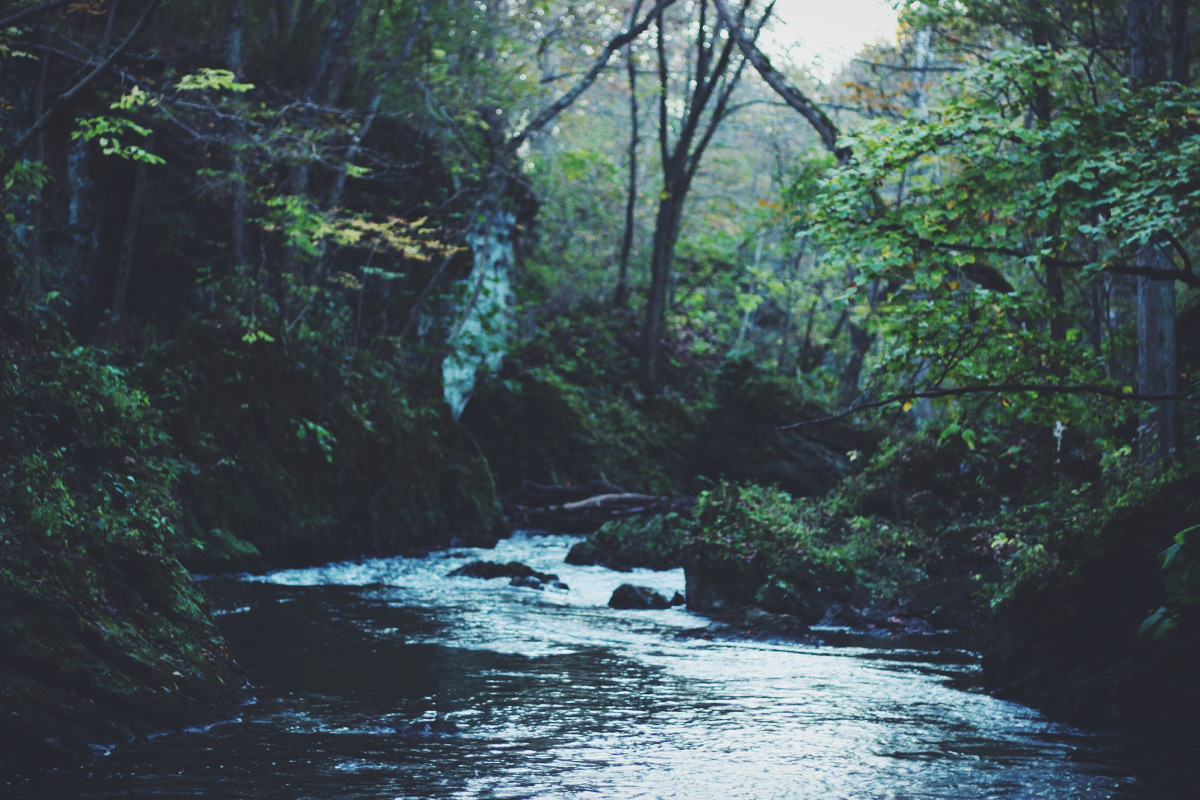
\includegraphics[width=\linewidth]{stream}
    \missingfigure{Insert sankey diagram}
    \caption{%
        {\bf HBN-POD2 data provenance}:
        Imaging data for \num{2747} subjects, aged 5-21 years and collected at four
        sites in the New York City area, was made available through the
        Functional Connectomes Project and the International Neuroimaging
        Data-Sharing Initiative (FCP-INDI).
        %
        These data were curated for compliance to the BIDS specification
        \cite{gorgolewski2016-lh} and availability of imaging metadata in json
        format. \num{2615} subjects met this specification.
        %
        Imaging data was preprocessed using \emph{QSIPrep} \cite{cieslak2021-iq}
        to group, distortion correct, motion correct, denoise, coregister and
        resample MRI scans. Of the BIDS curated subjects, \num{2136} subjects
        passed this step, with the majority of failures coming from subjects
        with missing dMRI scans.
        %
        Expert raters assigned QC scores to \num{200} of these participants,
        creating a ``gold standard'' QC subset. Community raters then assigned
        binary QC ratings to a superset of the gold standard containing
        \num{1653} participants. An image classification algorithm was trained
        on a combination of automated QC metrics from QSIPrep and community
        scientist reviews to ``extend'' the expert ratings to the community
        science subset.  Finally, a deep learning QC model was trained on the
        community science subset to assign QC scores to the entire dataset and
        to future releases from HBN.
        %
        The HBN-POD2 dataset, including QC ratings, is openly available through
        FCP-INDI.
    }
    \label{fig:hbn-sankey}
\end{figure}

To achieve the QC aim of the project, we adopted a hybrid QC approach that
combines expert rating, community science\footnote{%
    While the legacy term ``citizen science'' evokes a sense of civic duty in
    scientific engagement, it can be limiting by creating a barrier for
    community members who want to contribute to science but may not be U.S.
    citizens. In this manuscript we use the more modern ``community science''
    term.
}, and deep learning, drawing on the success of a previous application in
assessing the quality of HBN's structural MRI data \cite{keshavan2019-er}.
This method
\begin{enumerate*}[%
    label=(\roman*),%
    before={{ }},%
    itemjoin={{, }},%
    itemjoin*={{ and }}]
    \item starts with dMRI expert raters labelling a small subset of subjects,
    the ``gold standard'' dataset
    \item amplifies these labels using a community science web application to
    extend expert ratings to a much larger subset of the data, the community
    science subset
    \item trains a deep learning model on the community science subset to
    predict expert decisions on the entire dataset.
\end{enumerate*}

\subsection*{Expert quality control}

To create the gold standard dataset, we first created \emph{dmriprep-viewer}, a
dMRI data viewer and QC rating web application to display \emph{QSIPrep} outputs
and collect expert ratings \cite{richie-halford2021-viewer}.  We recruited six
dMRI experts to rate a 200-participant subset of the HBN-POD2 data using
extensive visual examination of each subjects dMRI data, including the diffusion
weighting imaging (DWI) time series itself, a plot of motion parameters through
the DWI scan, and full 3D volumes depicting
\begin{enumerate*}[%
    label=(\roman*),%
    before={{ }},%
    itemjoin={{, }},%
    itemjoin*={{ and }}]
    \item the brain mask and $b=0$ to T1w registration
    \item a diffusion tensor imaging (DTI) tensor fractional anisotropy (FA)
    model visualized over the $b=0$ volume.
\end{enumerate*}
The experts rated subjects using a five-point scale with ratings of ``definitely
fail,'' ``probably fail,'' ``unsure,'' ``probably pass,'' and ``definitely
pass.'' Figure \ref{fig:expert-qc:scatter} shows the distribution of expert
ratings and the relationship between the mean expert ratings and some of the
automated QC metrics output by \emph{QSIPrep}: neighboring DWI correlation (NDC)
\cite{yeh2019-kb}, maximum relative translation, and number of outlier slices.
NDC characterizes the pairwise spatial correlation between pairs of DWI volumes
that sample neighboring points in $q$-space. Since lower values indicate reduced
data quality, it is reassuring that NDC correlates directly with expert rating.
Conversely, high relative translation and a high number of motion outlier slices
reflect poor data quality and so these metrics are inversely related to mean
expert rating.

In addition to agreeing qualitatively with \emph{QSIPrep}'s automated QC
metrics, the expert raters also agreed with each other. To demonstrate
inter-rater reliability (IRR), in Figure \ref{fig:expert-qc:irr} we show the
pairwise Cohen's $\kappa$ \cite{di_eugenio2004-bb} for each pair of expert
raters as well as an additional XGB rater which we describe in the next
subsection.

In addition to the pairwise $\kappa$, we also present the intra-class
correlation (ICC) \cite{hallgren2012-ze} as a measure of IRR.  ICC3 and ICC3k
are appropriate variants of ICC when a fixed set of $k$ raters rate each subject
(i.e. a fully crossed design), which is what we have for HBN-POD2. When all
subjects are coded by multiple raters and the average of their ratings is used
for hypothesis testing, ICC3k is appropriate.  When a subset of subjects is
coded by multiple raters and the reliability of their ratings is meant to
generalize to other subjects rated by only one coder, the single-measure ICC3
must be used. The high ICC3k value for each expert rater entitles us to use the
mean expert rating as training data for the XGB algorithm.  And the high ICC
value after inclusion of the XGB model entitles us to treat XGB as a seventh
rater, thereby extending the expert ratings to the entire community science
subset.

\begin{figure}[ht]
    \begin{subfigure}{.5\textwidth}
    \centering
    % \includegraphics[width=.8\linewidth]{image_file_name}
    \missingfigure{Insert QC metric scatterplots}
    \caption{}
    \label{fig:expert-qc:scatter}
    \end{subfigure}
    \begin{subfigure}{.5\textwidth}
    \centering
    % \includegraphics[width=.8\linewidth]{image_file_name}
    \missingfigure{Insert expert rater IRR}
    \caption{}
    \label{fig:expert-qc:irr}
    \end{subfigure}
    \caption{%
        {\bf Expert QC results}:
        Six dMRI experts rated a subset of \num{200} subjects.
        \textbf{(a)} Experts agree with \emph{QSIPrep}'s automated QC metrics.
        Here we show associations between the expert QC rating and the
        \emph{QSIPrep} metrics neighboring diffusion-weighted imaging
        correlation (NDC) \cite{yeh2019-kb}, maximum relative translation, and
        number of outlier slices. As expected, NDC is directly correlated with expert rating while
        the other two metrics are inversely correlated with expert rating.
        %
        \textbf{(b)} Experts agree with each other. Here we show the pairwise
        Cohen's $\kappa$ measure of inter-rater reliability.  One can also use
        interclass correlation to demonstrate interrater reliability. The expert
        raters achieved an $\textbf{ICC3k} = 0.930 (95\% CI: [0.91, 0.94])$,
        $\textbf{ICC3} = 0.688 (95\% CI: [0.64, 0.74])$, $\langle \kappa \rangle
        = 0.648$.  We trained a gradient boosting model (XGB) to predict expert
        ratings based on community science ratings and automated QC metrics,
        obtaining a cross-validated ROC-AUC of $0.96 \pm 0.01$. Treating
        XGB as a seventh expert rater, preserves inter-rater reliability:
        $\textbf{ICC3k} = 0.945 (95\% CI: [0.93, 0.96])$, $\textbf{ICC3} = 0.709
        (95\% CI: [0.66, 0.75])$.  This entitles us to extend it's ratings to
        the community science dataset.
    }
    \label{fig:expert-qc}
\end{figure}

\subsection*{Community science quality control}

Although the expert raters achieved an acceptable inter-rater reliability and
yielded intuitive associations with \emph{QSIPrep}'s automated QC metrics,
generating expert QC labels for the entire HBN-POD2 dataset would be
prohibitively time consuming. To assess the image quality of the remaining
subjects, we released \emph{Fibr} (\url{https://fibr.dev}), a community science
web application in which users assign binary pass/fail labels assessing the
quality of horizonal slice tensor FA images. That is, \emph{Fibr} users saw
individual slices or an animated sequence of slices taken from the entire tensor
FA volume that the expert raters saw. The \emph{Fibr} users therefore saw only a
subset of the imaging data that the dMRI experts had access to. In total,
\num{374} community scientists provided \num{587778} ratings for a mean of $>50$
ratings per slice (or $>200$ ratings per subject). Of these, \num{145} raters
provided $>3,000$ votes each and are included as co-authors on this paper.

We then trained a gradient boosting model \cite{chen2016-eb} to predict expert
scores based on a combination of community science ratings and automated QSIPrep
QC metrics. We refer to this model as XGB.  To clarify the contributions of the
automated QC metrics and the community science raters, we trained two additional
gradient boosting models
\begin{enumerate*}[%
    label=(\roman*),%
    before=\unskip{: },%
    itemjoin={{, }},%
    itemjoin*={{ and }}]
    \item one trained only on the automated \emph{QSIPrep} QC metrics, which we
    call XGB-q
    \item one trained on only the \emph{Fibr} ratings, which we call XGB-f.
\end{enumerate*}
XGB-f may be viewed as a data-driven weighting of community scientists' ratings,
while XGB-q may be viewed as a generalization of QC metric exclusion criteria.
\arhtodo{%
    Add reference to paper showing the basic QC metric exclusion does about as
    good as braindr ratings for sMRI.
}
In Figure \ref{fig:fibr-qc:scatter}, we show the associations between the mean
expert rating and both the mean \emph{Fibr} rating and the XGB predictions.  The
unadjusted \emph{Fibr} ratings are overly optimistic; on average, community
scientists are not as critical as the expert raters. The XGB predictions remedy
this by
\begin{enumerate*}[%
    label=(\roman*),%
    before={{ }},%
    itemjoin={{, }},%
    itemjoin*={{ and }}]
    \item incorporating automated QC metrics from \emph{QSIPrep}
    \item weighting the contribution of \emph{Fibr} raters who agree more with
    the experts on the training set.
\end{enumerate*}
Figure \ref{fig:fibr-qc:roc} depicts the ROC curves for the XGB, XGB-q, and
XGB-f models.
XGB attains a cross validated area under the receiver operating curve (ROC-AUC) of
$0.96 \pm 0.01$ on the ``gold standard,'' where the $\pm$ indicates the standard
deviation of scores from repeated $k$-fold cross-validation.
In contrast, XGB-q attained an ROC-AUC of $0.91 \pm 0.03$ and XGB-f achieved an
ROC-AUC of $0.84 \pm 0.04$.
The enhanced performance of XGB-q over XGB-f shows that community scientists
alone are not as good as automated metrics at predicting expert ratings. And
yet, the increased performance of XGB over XGB-q demonstrates that there is
additional image quality information to be gained by visual inspecting dMRI
data.

\begin{figure}[ht]
    \begin{subfigure}{.5\textwidth}
    \centering
    % \includegraphics[width=.8\linewidth]{image_file_name}
    \missingfigure{Insert scatterplot of expert ratings with fibr avg and XGB output.}
    \caption{}
    \label{fig:fibr-qc:scatter}
    \end{subfigure}
    \begin{subfigure}{.5\textwidth}
    \centering
    % \includegraphics[width=.8\linewidth]{image_file_name}
    \missingfigure{Insert ROC curve of XGB models}
    \caption{}
    \label{fig:fibr-qc:roc}
    \end{subfigure}
    \caption{%
        {\bf Community science predictions of the expert ratings}:
        \textbf{(a)} Scatterplots showing the relationship between mean expert
        rating and both mean \emph{Fibr} rating (left) and XGB prediction
        (right). \emph{Fibr} raters overestimate the quality of images compared
        to expert raters. But the XGB prediction compensates for this by
        incorporating automated QC metrics and weighting more valuable
        \emph{Fibr} raters.
        %
        \textbf{(b)} ROC curves for the XGB, XGB-q, and XGB-f models.
    }
    \label{fig:fibr-qc}
\end{figure}

\subsection*{Automated QC labelling through deep learning}

The XGB ``rater'' does a good job of extending QC ratings to the entire
community science subset, but requires \emph{Fibr} scores. Without community
science ratings, it would fall back on the suboptimal XGB-q prediction. Instead,
we would like a fully automated QC approach that can be readily applied to new
data releases from HBN. We therefore trained a deep convolution neural network
to predict the XGB ratings from \emph{QSIPrep} outputs alone.

\arhtodo{
    Compute attribution masks from integrated gradients for select subjects (high
    consensus pass or fail)
}

\subsection*{So what?}

\arhtodo{
    Show QC bin tract profiles.

    Add effect of QC cutoff on age prediction from tract profiles.

    Try effect of QC cutoff on SES prediction from tract profiles.
}

\section*{Discussion}

We present HBN-POD2, one of the largest youth diffusion imaging datasets with
derived measures currently available. It is openly available and complies with
the current draft of the BIDS diffusion derivative specification. It will grow
continuously as the HBN study acquires more data, eventually reaching its
\num{10000} subject goal. The data is amenable to many different analyses,
including tractometry \cite{yeatman2012-rc}, graph theoretical analysis
\cite{yeh2020-nu}, and combinations with functional data for the same subjects.
The availability of standardized preprocessed diffusion data will allow
researchers to create and test hypotheses on the white matter properties
underlying behavior and disease, from reading and math acquisition to childhood
adversity and mental health. As such, this dataset will accelerate discovery at
the nexus of structural connectivity and neurodevelopmental and learning
disorders.

\subsection*{Standardized preprocessing reduces burden on downstream researchers}

\subsection*{Data sharing increases data value}

\subsection*{Limitations}

\subsection*{Future work}

\section*{Methods}

Inputs for this study consisted of MRI data from the Healthy Brain Network
pediatric mental health study \cite{alexander2017-yc}, containing dMRI data from
\num{2747} subjects with ages 5-21. These data were measured using a
\qty{1.5}{\tesla} Siemens mobile scanner on Staten Island (SI) and three fixed
\qty{3}{\tesla} Siemens MRI scanners at sites in the New York area: Rutgers
University Brain Imaging Center (RUBIC), the CitiGroup Cornell Brain Imaging
Center (CBIC), and the City University of New York Advanced Science Research
Center (CUNY). Informed consent was obtained from each participant aged 18 or
older. For participants younger than 18, written consent was obtained from their
legal guardians and written assent was obtained from the participant. Voxel
resolution was \qtyproduct{1.8 x 1.8 x 1.8}{\mm} with \num{64} non-colinear
directions measured for each of $b=1000$ \unit{\second \per \mm^{2}} and
$b=2000$ \unit{\second \per \mm^{2}}.

\subsection*{BIDS curation}

We curated the imaging metadata for \num{2615} of the \num{2747} currently
available HBN subjects. Using dcm2bids and custom scripts, we conformed the data
to the Brain Imaging Data Structure (BIDS; \cite{gorgolewski2016-lh})
specification.  The BIDS-curated dataset is available on FCP-INDI and can be
accessed via AWS S3 at \url{s3://fcp-indi/data/Projects/HBN/BIDS_curated/}.

\mctodo[inline]{Add more BIDS curation information}

\subsection*{Preprocessing}

We performed dMRI preprocessing on \num{2136} subjects, using \emph{QSIPrep}
\cite{cieslak2021-iq} 0.12.1, which is based on \emph{Nipype} 1.5.1
\cite{nipype1,nipype2}, RRID:SCR\_002502. \emph{QSIPrep} a robust and scalable
pipeline to group, distortion correct, motion correct, denoise, coregister and
resample MRI scans.  In total, \num{417} subjects failed this preprocessing
step, largely due to missing dMRI files. In keeping with the BIDS specification,
the preprocessed dataset is available as a derivative dataset within the
BIDS-curated dataset and can be access on AWS S3 at
\url{s3://fcp-indi/data/Projects/HBN/BIDS_curated/derivatives/qsiprep/}.
\emph{QSIPrep} fosters reproducibility by automatically generating thorough
methods boilerplate for later use in scientific publications, which we use for
the remainder of this subsection to document each preprocessing step.

\begin{itemize}

\item {\it Anatomical data preprocessing}
The T1-weighted (T1w) image was corrected for intensity non-uniformity (INU)
using \texttt{N4BiasFieldCorrection} \cite{n4} (ANTs 2.3.1), and used as
T1w-reference throughout the workflow. The T1w-reference was then skull-stripped
using \texttt{antsBrainExtraction.sh} (ANTs 2.3.1), using OASIS as target
template. Spatial normalization to the ICBM 152 Nonlinear Asymmetrical template
version 2009c \cite{mni}, RRID:SCR\_008796 was performed through nonlinear
registration with \texttt{antsRegistration} \cite{ants}, ANTs 2.3.1,
RRID:SCR\_004757, using brain-extracted versions of both T1w volume and
template. Brain tissue segmentation of cerebrospinal fluid (CSF), white-matter
(WM) and gray-matter (GM) was performed on the brain-extracted T1w using
\texttt{FAST} \cite{fsl_fast}, FSL 6.0.3:b862cdd5, RRID:SCR\_002823.

\item {\it Diffusion data preprocessing}

Any images with a $b$-value less than \qty{100}{\second \per \mm^{2}} were treated
as a $b=0$ image. MP-PCA denoising as implemented in MRtrix3's
\texttt{dwidenoise}\cite{dwidenoise1} was applied with a 5-voxel window. After
MP-PCA, B1 field inhomogeneity was corrected using \texttt{dwibiascorrect} from
MRtrix3 with the N4 algorithm \cite{n4}.  After B1 bias correction, the mean
intensity of the DWI series was adjusted so all the mean intensity of the $b=0$
images matched across eachseparate DWI scanning sequence.

FSL (version 6.0.3:b862cdd5)'s eddy was used for head motion correction
and Eddy current correction \cite{anderssoneddy}. Eddy was configured
with a \(q\)-space smoothing factor of 10, a total of 5 iterations, and
1000 voxels used to estimate hyperparameters. A linear first level model
and a linear second level model were used to characterize Eddy
current-related spatial distortion. \(q\)-space coordinates were
forcefully assigned to shells. Field offset was attempted to be
separated from subject movement. Shells were aligned post-eddy. Eddy's
outlier replacement was run \cite{eddyrepol}. Data were grouped by
slice, only including values from slices determined to contain at least
\num{250} intracerebral voxels. Groups deviating by more than four standard
deviations from the prediction had their data replaced with imputed
values. Data was collected with reversed phase-encode blips, resulting
in pairs of images with distortions going in opposite directions. Here,
$b=0$ reference images with reversed phase encoding directions were used
along with an equal number of $b=0$ images extracted from the DWI scans.
From these pairs the susceptibility-induced off-resonance field was
estimated using a method similar to that described in \cite{topup}. The
fieldmaps were ultimately incorporated into the Eddy current and head
motion correction interpolation. Final interpolation was performed using
the \texttt{jac} method.

Several confounding time-series were calculated based on the
\emph{preprocessed DWI}: framewise displacement (FD) using the implementation
in \emph{Nipype} following the definitions by \cite{power_fd_dvars}. The DWI
time-series were resampled to ACPC, generating a \emph{preprocessed DWI run
in ACPC space}.

\item {\it MRtrix3 Reconstruction}

Reconstruction was performed using \emph{QSIprep} 0.12.1. Multi-tissue fiber
response functions were estimated using the dhollander algorithm. FODs were
estimated via constrained spherical deconvolution (CSD, \cite{originalcsd,
tournier2008csd}) using an unsupervised multi-tissue method
\cite{dhollander2019response, dhollander2016unsupervised}. Reconstruction was
done using MRtrix3 \cite{mrtrix3}. FODs were intensity-normalized using
mtnormalize \cite{mtnormalize}.

\end{itemize}

Many internal operations of \emph{QSIPrep} use \emph{Nilearn} 0.6.2
\cite{nilearn}, RRID:SCR\_001362 and \emph{DIPY} \cite{dipy}. For more details
of the pipeline, see
\href{https://qsiprep.readthedocs.io/en/latest/workflows.html}{the section
corresponding to workflows in \emph{QSIPrep}'s documentation}.

\subsection*{Cloud-based distributed preprocessing}

\arhtodo[inline]{Add information on cloudknot}
Using a previously developed cloud-computing library
\cite{richie-halford2018-kv} to parallelize the preprocessing over individual
subjects on spot instances in the Amazon Web Services Batch service, this dMRI
preprocessing cost less than \textdollar1.00 per subject.

\subsection*{Expert quality control}

The expert QC ``gold standard'' subset was created by randomly selecting 200
subjects from the preprocessed dataset, sampled such that the proportional site
distribution in the gold standard subset matched that of the preprocessed
dataset.

We created a web application for expert quality control of preprocessed dMRI,
called \emph{dmriprep-viewer} \cite{richie-halford2021-viewer}.
\comment[inline]{%
    We might change the name of the viewer now that it's going to be modality
    agnostic.%
}

\arhtodo[inline]{%
    Add information on dmriprep-viewer, the QC instruction video, and the expert
    QC procedures
}

\subsection*{Community scientist quality control}

The community science web application is based on the
\href{https://swipesforscience.org/}{SwipesForScience framework}, which
generates a web application for community science given an open repository of
images to be labelled and a configuration file.
After a brief tutorial, community scientists provided binary pass/fail ratings
based on the directionally-colorized fractional anisotropy from DTI of each
subject's preprocessed dMRI data. These community scientist ratings were then
combined with expert ratings to train a neural network to assign a quality
control (QC) rating to each subject.

\subsection*{Deep learning to predict quality control}

\begin{itemize}
    \item Show architecture and point to the CT scan paper \cite{zunair2020-bs}.
    \item Two model types
    \item Data format (4-channels + QSIPrep QC metric input)
    \item Learning curves
\end{itemize}

\subsection*{Brain age prediction}

\bibliography{hbn-pod2}

\section*{Acknowledgements}

We would like to thank Anisha Keshavan for useful discussions of community
science and web-based quality control. This manuscript was prepared using a
limited access dataset obtained from the Child Mind Institute Biobank, The
Healthy Brain Network dataset. This manuscript reflects the views of the authors
and does not necessarily reflect the opinions or views of the Child Mind
Institute.
\alltodo[inline]{Add grant numbers.}

\section*{Author contributions statement}

The first author named is the corresponding author. The last two authors named
share senior authorship. The first two authors named share lead authorship.  The
next ten authors' contributions extended beyond providing community science
annotations and are listed in alphabetical order. All other authors are Fibr
community scientists and are listed in descending order of the number of QC
labels they produced.

\alltodo[inline]{Please add your initials here as appropriate}

We describe contributions to the paper using the CRediT taxonomy \cite{brand2015-vd}:
\begin{itemize}
    \item Conceptualization: A.R-H., A.R., T.S., and M.C.;
    \item Methodology: A.R-H. and A.R.;
    \item Software: A.R-H. and M.C.;
    \item Validation: ;
    \item Formal Analysis: A.R-H. and M.C.;
    \item Investigation: A.R-H. and M.C.;
    \item Resources: M.M.;
    \item Data curation: M.C. and L.A.;
    \item Writing – Original Draft: A.R-H. and A.R.;
    \item Writing – Review \& Editing: ;
    \item Visualization: A.R-H.;
    \item Supervision: A.R. and T.S.;
    \item Project Administration: A.R-H. and A.R.;
    \item Funding Acquisition: A.R. and T.S.
\end{itemize}

\section*{Additional information}

To include, in this order: \textbf{Accession codes} (where applicable);
\textbf{Competing interests} (mandatory statement).

The corresponding author is responsible for submitting a
\href{http://www.nature.com/srep/policies/index.html#competing}{competing
interests statement} on behalf of all authors of the paper. This statement must
be included in the submitted article file.

\arhtodo[inline]{Add accession codes and competing interests statement.}

% \begin{figure}[ht]
% \centering
% 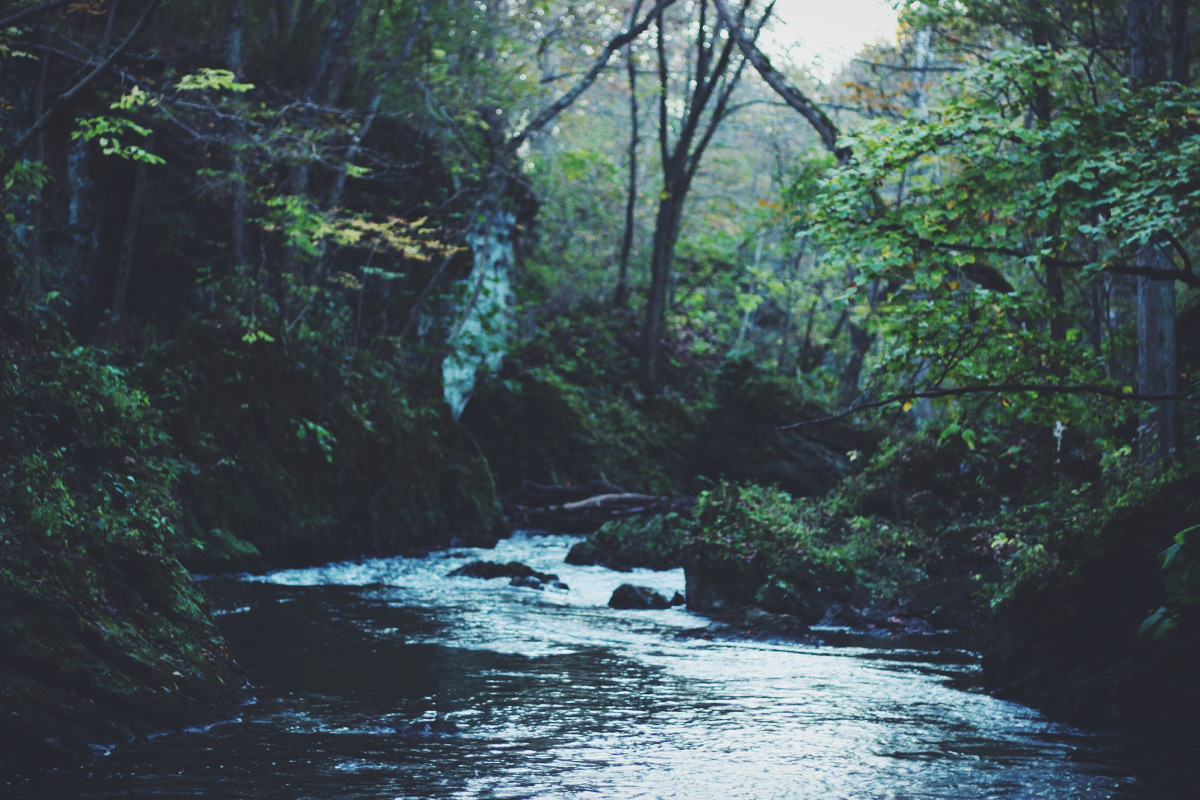
\includegraphics[width=\linewidth]{stream}
% \caption{Legend (350 words max). Example legend text.}
% \label{fig:stream}
% \end{figure}

% \begin{table}[ht]
% \centering
% \begin{tabular}{|l|l|l|}
% \hline
% Condition & n & p \\
% \hline
% A & 5 & 0.1 \\
% \hline
% B & 10 & 0.01 \\
% \hline
% \end{tabular}
% \caption{\label{tab:example}Legend (350 words max). Example legend text.}
% \end{table}

% Figures and tables can be referenced in LaTeX using the ref command, e.g. Figure \ref{fig:stream} and Table \ref{tab:example}.

\end{document}